\newcommand{\ClassPath}{../VIU_TFM_LaTeX_template}
\documentclass{\ClassPath/viu-tfm-template}
\usepackage{multicol}

\definecolor{maincolor}{HTML}{f25416}

%--------------------------------------------------------------------------
% Definiciones necesarias Modifica con tus datos
%--------------------------------------------------------------------------
\def\nombre{Gómez Olivencia, Rubén}
\def\dni{78910013-A}
\def\titulo{Aplicaciones de gestión de proyectos:\linebreak\linebreak Diagrama de Gantt}
\def\titulacion{Máster Universitario en Desarrollo de Aplicaciones y Servicios Web}
\def\curso{2022-2023}

%Los siguientes son opcionales: si no se ponen, la portada cambia un poco. Ideal para escribir artículos/trabajos cortos
\def\dirige{}
\def\convocatoria{}
\def\asignatura{Gestión de proyectos en entornos ágiles}


% importar fichero de Bibliografía
%\addbibresource{Actividad_1.bib}

\begin{document}
    \graphicspath{{../VIU_TFM_LaTeX_template/}}

    \coverpage

    \tableofcontents

\chapter{Introducción}

A la hora de gestionar proyectos hoy en día se hace uso de las denominadas metodologías ágiles. Es cierto que estas nuevas metodologías han aportado flexibilidad y mejoras, pero eso no quita para que metodologías previas (denominadas predictivas) como los \href{https://es.wikipedia.org/wiki/Diagrama_de_Gantt}{diagramas de Gantt} puedan seguir aportando gran valor en etapas iniciales en la gestión de proyectos.

Es por eso que a lo largo de este documento se van a analizar distintos programas que nos van a permitir la gestión inicial de un proyecto haciendo uso de los diagramas de Gantt.


\chapter{Software de gestión: Diagramas de Gantt}
A la hora de gestionar un proyecto haciendo uso de los diagramas de Gantt hay que decidir qué \textit{software} se va a utilizar para llevar a cabo la planificación.

Este software nos debe permitir gestionar un equipo, crear las distintas etapas por las que el proyecto va a pasar, crear dependencias de tareas... Es importante realizar una buena elección, que se ajuste a las necesidades que vamos a necesitar, para que no suponga una carga o un gasto de tiempo el utilizarlo.

Es por ello que se va a realizar un análisis de distintos programas, en los que se expondrán las ventajas de cada uno de ellos y para finalizar se expondrá por cuál de ellos nos hemos decantado.

A la hora de realizar el análisis y la elección se han tenido en cuenta los siguientes aspectos:
\begin{itemize}
    \item Mejor que sea \textbf{Software Libre}. Debido a las ventajas del Software Libre, nos permitirá realizar modificaciones en caso de que sea necesario para poder adaptarlo a las necesidades propias en caso de que falte alguna característica.

    \item Que sea un proyecto que \textbf{se mantenga “vivo”}. Teniendo en cuenta el punto anterior, ya sea para poder realizar una modificación propia o pedirle al desarrollador la posibilidad de implementarla, es necesario que el software se siga manteniendo y desarrollando. Aparte, eso también significará que su uso está extendido.
    \item Que sea \textbf{multiplataforma}, \textbf{o desarrollado en entorno web}. Debido a que en el equipo se hace uso de distintos sistemas operativos, es conveniente que el programa elegido se pueda utilizar en distintos sistemas operativos.

    En caso de que sea un desarrollo web, evitaríamos ese problema, pero sería interesante que tuviese sistema de control de usuarios. También es recomendable poder contar con la posibilidad de tener el sistema en nuestros propios servidores.

    \item Uso de \textbf{estándares abiertos}, sobre todo a la hora de exportar el diagrama. Suele ser lo habitual con el Software Libre, pero es recomendable saber que lo realizado se puede exportar en un formato libre que posteriormente pueda ser abierto con otro programa, por si en el futuro se decide cambiar de programa.
\end{itemize}

Teniendo en cuenta estas características, nos aseguraremos que el software elegido no nos limita durante la gestión del proyecto, y que en caso de que así sea, se pueda cambiar rápidamente por una alternativa mejor.


\section{Análisis de software}

A continuación se va a realizar el análisis de distintas aplicaciones identificando algunas de sus características, ya sean ventajas o inconvenientes, para realizar una pequeña comparativa final.

En la \href{https://en.wikipedia.org/wiki/Comparison_of_project_management_software}{Wikipedia} existe una página de software de gestión de proyectos, que nos puede servir como una guía de inicio para empezar a buscar.

\subsection{Gantt Project}

\href{https://www.ganttproject.biz/}{Gantt Project} es una aplicación de escritorio multiplataforma que tiene una larga trayectoria a sus espaldas. Es Software Libre y está escrito en Java.

Entre las ventajas que se pueden destacar es que se pueden generar reportes en formato PDF y HTML, se puede importar y exportar a/desde Microsoft Project, tiene gestión de vacaciones y es Software Libre.


\begin{center}
    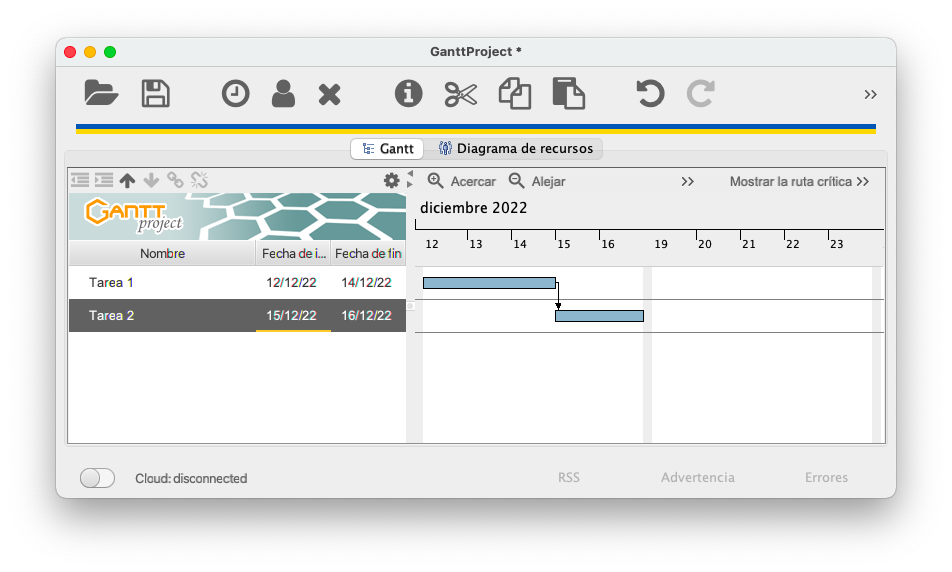
\includegraphics[width=0.7\linewidth]{img/ganttproject.png}
\end{center}

Como inconveniente se le puede poner que es una aplicación de escritorio, aunque tienen una opción de pago llamada “GanttProject Cloud” para modo colaborativo.

\subsection{Gnome Planner}
\href{https://wiki.gnome.org/Apps/Planner}{Gnome Planner} es otra aplicación de escritorio dentro del ecosistema del escritorio \href{https://www.gnome.org/}{Gnome}, muy conocido en el mundo GNU/Linux.

Esta aplicación a nivel visual, aunque es subjetivo, se puede decir que está más cuidada, y en caso de utilizar un escritorio Gnome, se integra perfectamente en lo que ya conocemos.

\begin{center}
    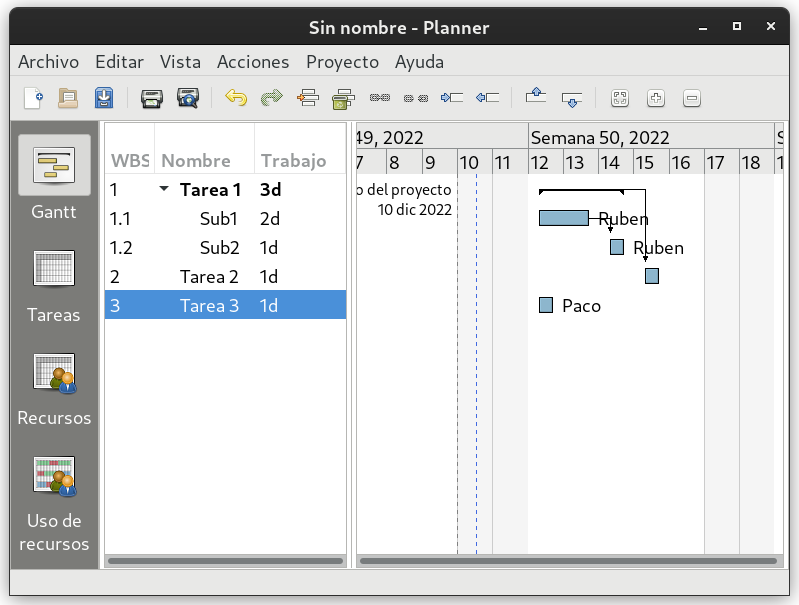
\includegraphics[width=0.7\linewidth]{img/planner.png}
\end{center}

Por otro lado, cuenta con la posibilidad de crear grupos de personas/recursos, y de manera sencilla se puede ver el listado de tareas completas y el estado de cada recurso, en qué está ocupado en el momento actual o si por el contrario está libre.

Al igual que sucede con la anterior aplicación, al ser una aplicación de escritorio limita el uso de distintos usuarios al mismo fichero/proyecto.


\subsection{Instagantt}
\href{https://instagantt.com/}{Instagantt} es una aplicación web para poder crear diagramas de Gantt que está enfocado para el gestor de proyectos \href{https://asana.com/es}{Asana}.


\begin{center}
    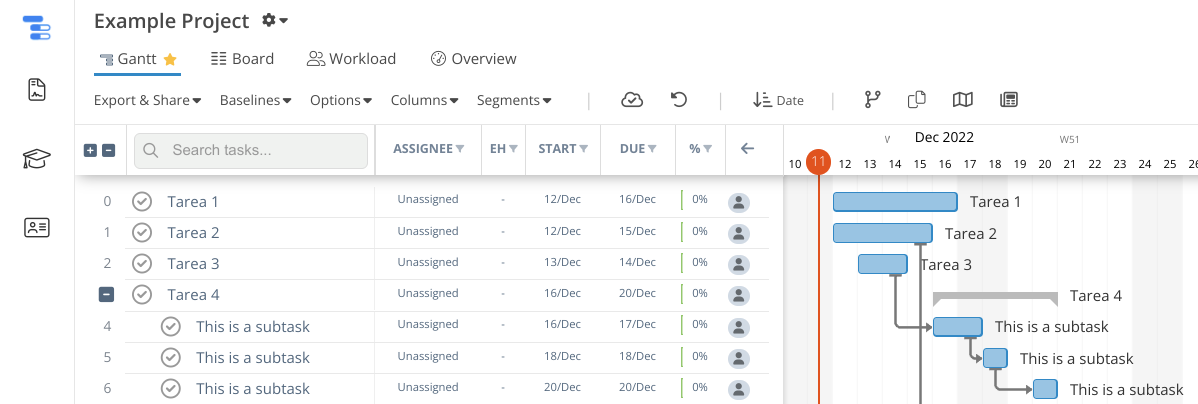
\includegraphics[frame,width=0.8\linewidth]{img/instagantt.png}
\end{center}

Instagantt tiene un periodo de prueba de 7 días, en los que se podrá hacer uso de él, pero después tiene un pago de suscripción de 7 dólares al mes para un único usuario, o 5 dólares por usuario/mes si queremos que se pueda utilizar de manera cooperativa.


\subsection{Redmine}

\href{https://www.redmine.org/}{Redmine} es un gestor de proyectos completo basado en web. Es Software Libre, está escrito en Ruby on Rails y es fácil de crear una instancia a través de contenedores Docker.

Al ser un gestor de proyectos completo tiene sus ventajas a la hora de utilizarlo dentro de una empresa, ya que desde una aplicación podemos crear incidencias, gestionar código fuente, referenciar modificaciones de código asociado a incidencias... Es una herramienta muy potente que para tener un histórico de todo lo realizado por los trabajadores y la empresa viene muy bien.

Por otro lado, su implantación no es sencilla ni rápida, ya que hay que dar de alta a los usuarios, crear distintos estados de las incidencias, crear flujos de trabajo, crear perfiles de usuarios sobre proyectos, asignarlos a usuarios...

\begin{center}
    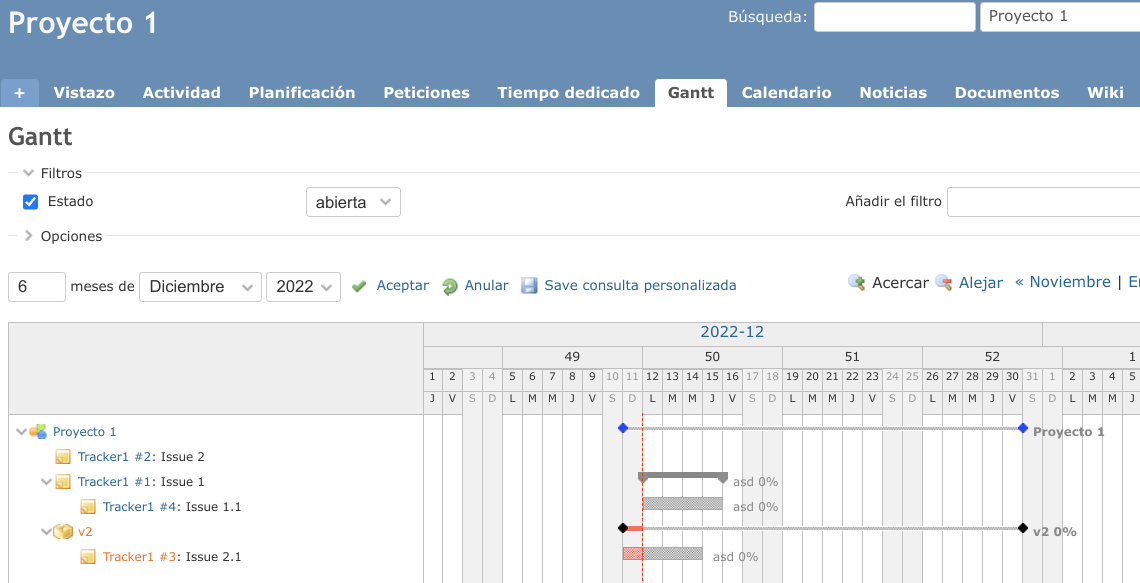
\includegraphics[frame,width=0.7\linewidth]{img/redmine.png}
\end{center}

Una vez superado lo mencionado anteriormente, como tendremos que haber ido creando las incidencias y asignarlas a los usuarios, la ventaja es que no sólo tendremos el diagrama de Gantt hecho, si no toda la gestión del proyecto, incidencias, asignaciones... Ya que todo se encuentra en la misma aplicación web.


\subsection{OpenProject}

Al igual que el caso anterior, \href{https://www.openproject.org/}{OpenProject} es un software web para la gestión de proyectos completos. También es Software Libre, también programado en Ruby on Rails, pero esta vez con la parte \textit{frontend} hecha en Angular.

Este software está pensado para el uso por parte de todos los integrantes de una empresa, para la creación de tareas, seguimiento... y levantar una instancia con Docker, una vez más,  resulta muy sencillo.

\begin{center}
    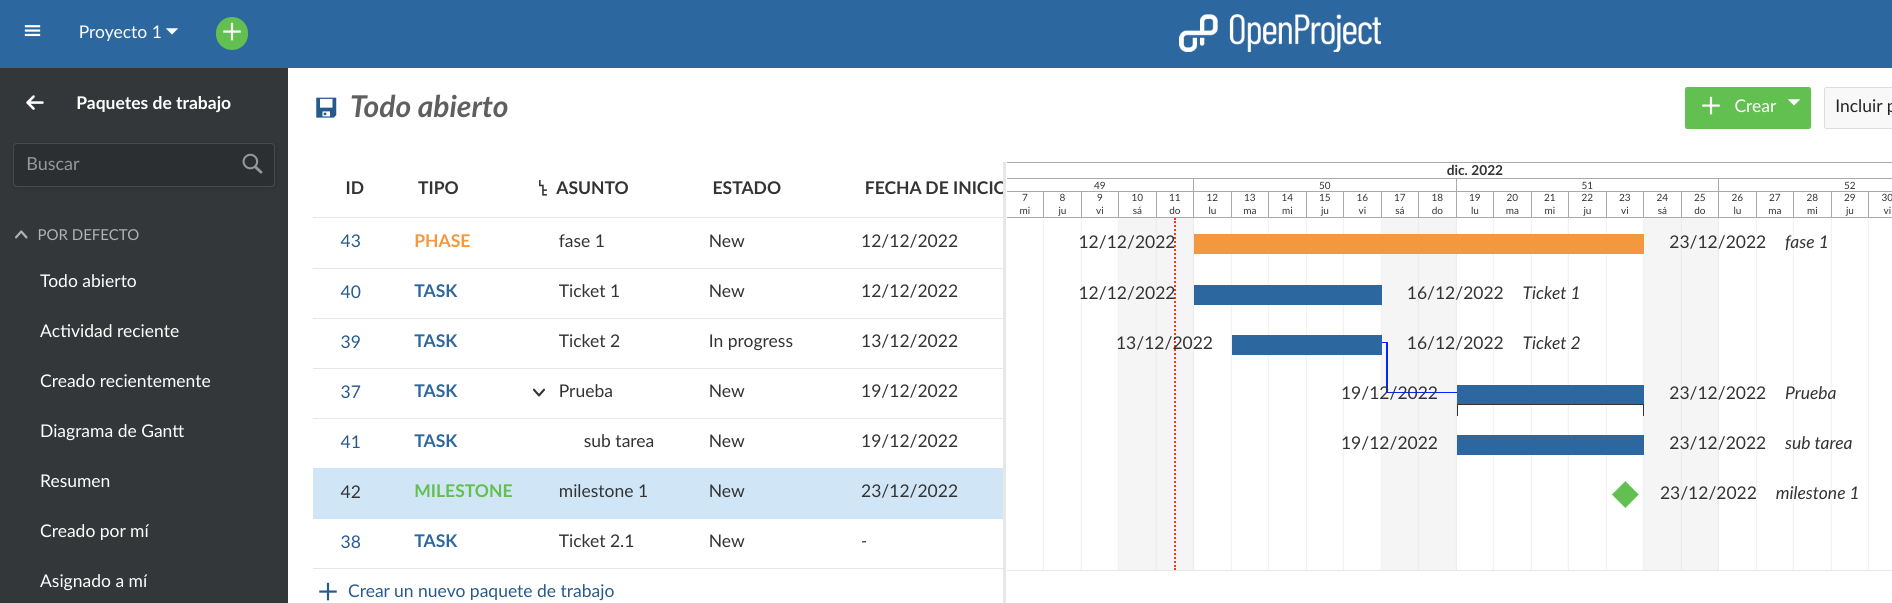
\includegraphics[frame,width=0.9\linewidth]{img/openproject.png}
\end{center}

Tal como sucedía con Redmine, hay que dar de alta a los usuarios, pero a la hora de crear las tareas, asignarlas, cambiar el estado de las mismas... es mucho más intuitivo. Ya existen estados pre-definidos, el relacionar tareas entre sí es mucho más sencillo, se pueden modificar fechas en el propio diagrama de Gantt, el aspecto visual está mucho más cuidado...

Tiene una versión “Enterprise” que cuenta con distintos añadidos, pero la versión libre es completamente funcional. El problema principal de esta aplicación es que abarca demasiado si sólo queremos crear un diagrama de Gantt.


\section{Comparativa}

A continuación, una pequeña tabla comparativa de las distintas aplicaciones analizadas:

\begin{yukitblrcol}{XXXXXX}
    & Gantt Project & Gnome Planner & Redmine & Open Project & Instagantt \\
    Software Libre & \checkmark & \checkmark & \checkmark & \checkmark & \times \\
    Multi usuario & Equipos de 2 gratis & \times & \checkmark & \checkmark & Pagando \\
    Multi plataforma & \checkmark & Linux / Windows & \checkmark & \checkmark & \checkmark \\
    Facilidad de uso & Fácil & Fácil & Complejo & Medio & Fácil \\
\end{yukitblrcol}


\section{Elección del software a utilizar}
Teniendo en cuenta que se ha analizando software muy diverso (unos que sólo permiten la creación de diagramas de Gantt y otros que son gestores de proyecto completos, con soporte de creación de incidencias, gestión de tiempo, usuarios...) hay que tener en cuenta las necesidades actuales, para “no matar moscas a cañonazos”.

Si necesitásemos la gestión completa de un proyecto, para tener control total de tiempos por empleados, creación de incidencias, gestión de las mismas, aparte de la creación del diagrama de Gantt, la mejor opción sería Open Project.

En cambio, las necesidades actuales lo único que abarcan es la creación de un diagrama de Gantt con la gestión de recursos, por lo que las funcionalidades que nos ofrece \textbf{Gantt Project} se ajustan perfectamente a lo que necesitamos.


\chapter{Creación del proyecto}
A la hora de crear el proyecto no había una idea clara, por lo que, como veremos más adelante, se hizo uso de parte de la planificación para hacer un \textit{brainstorming} y así decidir qué tipo de proyecto realizar para el TFM (trabajo fin de máster).

Al final se ha decidido crear un gestor de contraseñas y documentación sensible basado en una plataforma web creada con \href{https://angular.io/}{Angular} y que hará uso como \textit{backend} del sistema \href{https://www.vaultproject.io/}{Vault} de la empresa Hashicorp.


\chapter{Planificación}
Teniendo ya la idea del proyecto a realizar, el siguiente paso es detallar la planificación realizada para llevar a cabo el proyecto.

A continuación se van a detallar distintos apartados que se han tenido en cuenta durante la planificación

\section{Necesidad de recursos y roles}
Para llevar a cabo el proyecto se va a hacer uso de un equipo de máximo cinco trabajadores, y se puede considerar que todos tienen un rol multidisciplinar, ya que tienen experiencia en distintos ámbitos.

Esto nos va a permitir que todos ellos puedan desempeñar cualquier rol en cualquier momento a lo largo del proyecto, por lo que va a facilitar la labor de asignación de tareas, y hará que no exista “cuello de botella” por los conocimientos y/o experiencia que tengan.

También nos va a facilitar en caso de que en algún momento haya algún tipo de baja temporal o vacaciones no planificadas de último momento, ya que cualquiera podrá retomar la tarea dejada a medias.


\section{Tareas a realizar}

A la hora de realizar la planificación se han identificado las distintas tareas que deben realizarse para completar el proyecto. Para facilitar la ejecución y ordenación  se han agrupado de la siguiente manera:

\begin{itemize}
    \item \textbf{Brainstorming inicial}: Fase inicial del proyecto en la que el equipo al completo se dedicó a realizar una tormenta de ideas para analizar el tipo de proyecto que se quería realizar para el TFM.

    \item \textbf{Investigación}: Una vez decidido las ideas generales del proyecto, el equipo se ha dividido para realizar distintas investigaciones previas (de forma paralela) que son necesarias antes de comenzar con el desarrollo. Entre estas tareas se destacan:
    \begin{itemize}
        \item Entender cómo funciona la API de Vault.
        \item Crear concepto/boceto del interfaz web que va a contar la aplicación, al ser posible en HTML estático.
        \item Investigar distintos \textit{frameworks} web que se pueden utilizar para el desarrollo.
    \end{itemize}

    \item \textbf{Puesta en conjunto} de lo realizado en el punto anterior, y toma de decisiones de cómo se va a realizar el proyecto final.

    \item \textbf{Desarrollo del proyecto}. Este es el grupo que más actividades tiene y que más tiempo va a requerir de todo el proyecto.

    \item \textbf{Testeo}. Se ha creado un grupo en el que se han añadido distintas tareas para realizar tests de usabilidad, integración y test del conjunto en distintas etapas del proyecto.

    \item Para la \textbf{puesta en producción} del proyecto se han creado un par de tareas:
    \begin{itemize}
        \item Investigar distintos proveedores donde se puede desplegar la aplicación, teniendo en cuenta precio final/año y facilidad de usto.
        \item Tiempo de realizar el propio despliegue
    \end{itemize}

    \item Se han reservado diferentes etapas para realizar la \textbf{documentación}, ampliarla en caso necesario y comprobar que es correcta por parte de los desarrolladores. Esto es algo que no siempre se tiene en cuenta en el tiempo del proyecto.

    \item Para finalizar, la \textbf{presentación y entrega del proyecto}, que será el último paso a realizar del proyecto.
\end{itemize}

\section{Temporalización}
Para realizar el proyecto se contará con un máximo de 3 meses habiendo empezado el 12 de diciembre, y siendo la fecha de entrega el 13 de marzo del 2023.

Se ha tenido en cuenta los días festivos locales y nacionales donde están los desarrolladores, y también las vacaciones que ya estaban agendadas previamente.

Con todo ello, se ha conseguido reservar una semana entre la fecha estimada de finalización de la última tarea a realizar y la presentación. De esta manera, en caso de que surjan problemas, contaremos con varios días de margen.

\section{Diagrama final}

A continuación se va a mostrar la imagen del diagrama final completo, para hacernos una idea general de los distintos grupos que se han mencionado antes:

\begin{center}
    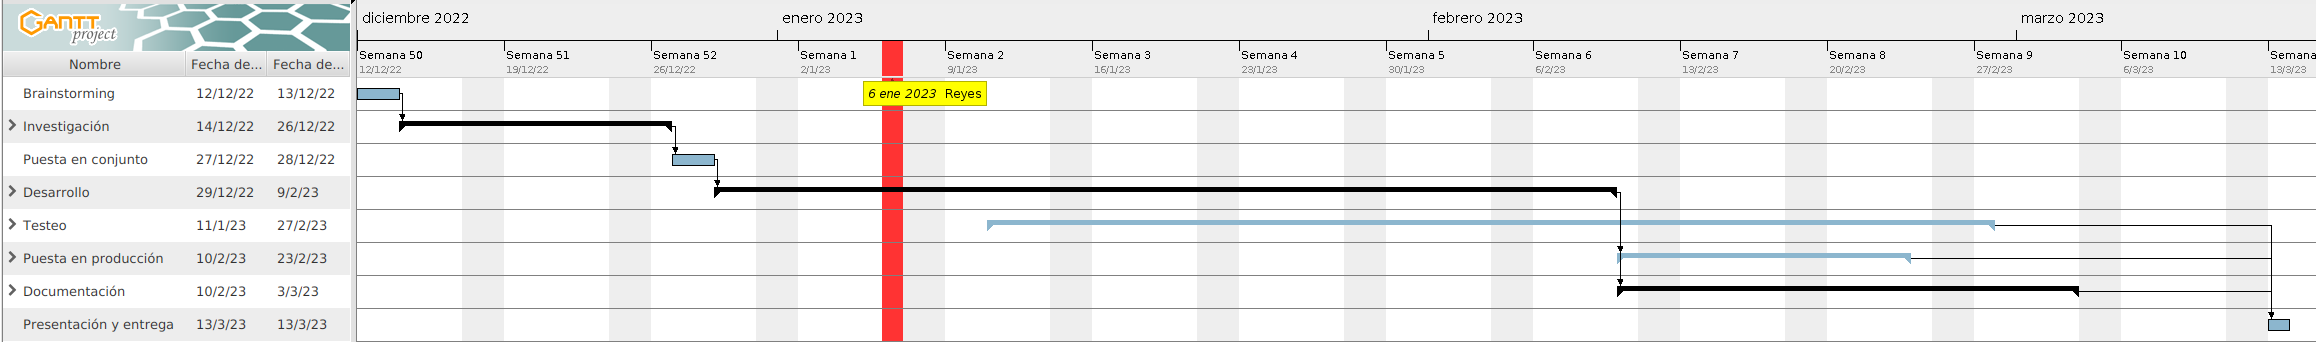
\includegraphics[frame,width=\linewidth]{img/diagrama.png}
\end{center}


Tras el diagrama general, se va a mostrar las tareas a realizar desplegadas, y mostrando quién va a ser el responsable (su nombre aparece entre llaves “\{\}”) de cada una de ellas y quiénes participarán en ellas.

También se puede ver el nombre de la tarea, junto con el número de días que se ha estimado que se van a necesitar. Encima de cada grafo de la tarea aparecen las fechas en las que se llevará a cabo, y debajo los participantes.

Tal como se ha comentado previamente, el proyecto comienza con un \textit{brainstorming} en el que participa todo el equipo para pensar el proyecto que se va a realizar.

Tras tomar la decisión de crear el “gestor de contraseñas y documentación sensible basado en una plataforma web”, entramos en una etapa de investigación. En esta etapa el equipo se divide para tratar de buscar el mejor framework web a utilizar, comenzar a hacer un boceto del interfaz de la aplicación y entender cómo funciona el sitema Vault y su API.

Tras esto, se dedican dos días para poner las ideas en común, y tomar las decisiones para continuar con el proyecto.

\begin{center}
    \vspace{-20pt}
    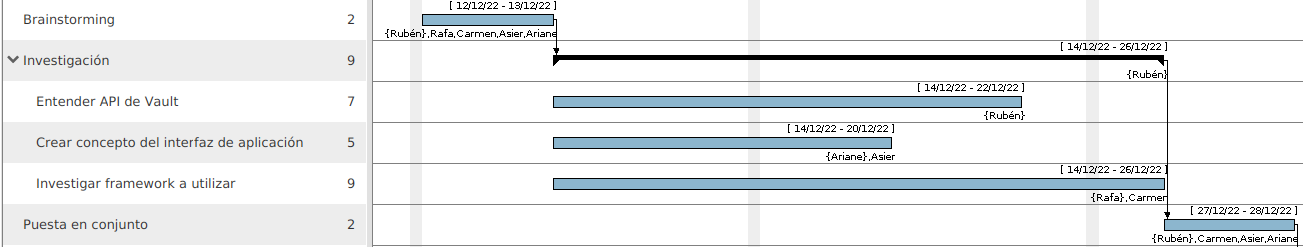
\includegraphics[frame,width=\linewidth]{img/gantt1.png}
    \vspace{-20pt}
\end{center}

Para cada una de las tareas se va a contar con un responsable propio, pero para cada agrupación de las mismas (como en el caso anterior de “Investigación”) va a haber un responsable “general” que va a ser Rubén Gómez.

Es por eso que a pesar de que él contará con sus propias tareas asignadas, se le reserva un porcentaje de tiempo para dedicar a conocer el estado general del resto de tareas y así que pueda planificar posibles modificaciones futuras.

La estimación siguiente es todo el proceso de desarrollo de la aplicación que se puede ver en el siguiente diagrama desplegado.

En este caso no todas las tareas se pueden paralelizar, ya que algunas son dependientes de otras y por tanto es necesario que estén realizadas para poder continuar.

La primera parte del desarrollo se puede dividir en crear la base del proyecto con las dependencias necesarias con el \textit{framework elegido}, desarrollar el interfaz web y crear las llamadas a la API de Vault necesarias.

Esta fase se va a mezclar con un testeo del interfaz web que es bloqueante (para ver si cumple con la usabilidad esperada) y con otra fase de integración.

\begin{center}
    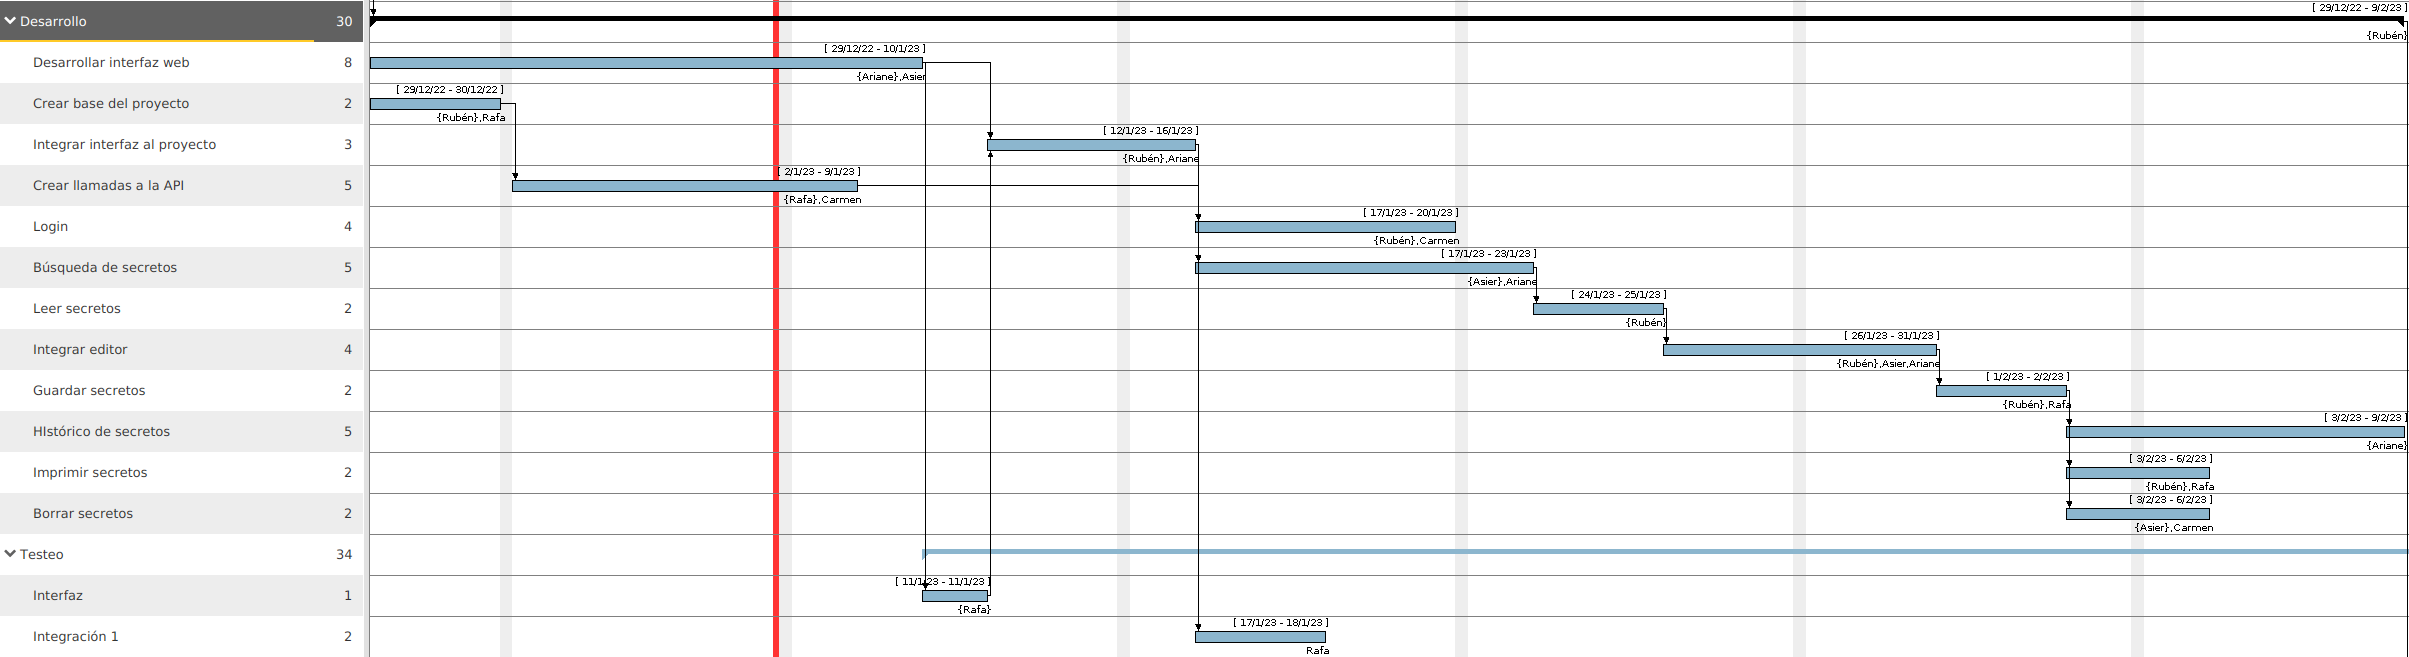
\includegraphics[frame,width=\linewidth]{img/gantt2.png}
\end{center}

El resto de tareas a realizar, están asignadas y paralelizadas lo máximo posible para así tratar de acortar el tiempo lo máximo posible.

La última parte del proyecto se puede dividir en dos grandes grupos, que son la puesta en producción y crear la documentación.

Aunque ya se tiene experiencia en Amazon AWS para poner servicios en producción, se ha decidido reservar 5 días para investigar posibles alternativas (ya sea otro proveedor cloud o un proveedor de servidores donde realizar la configuración por nuestra cuenta). En caso de que las tareas del desarrollo comiencen a sufrir retrasos, se podría optar por no realizar esta investigación, usar AWS, y así ganar esos días.

\begin{center}
    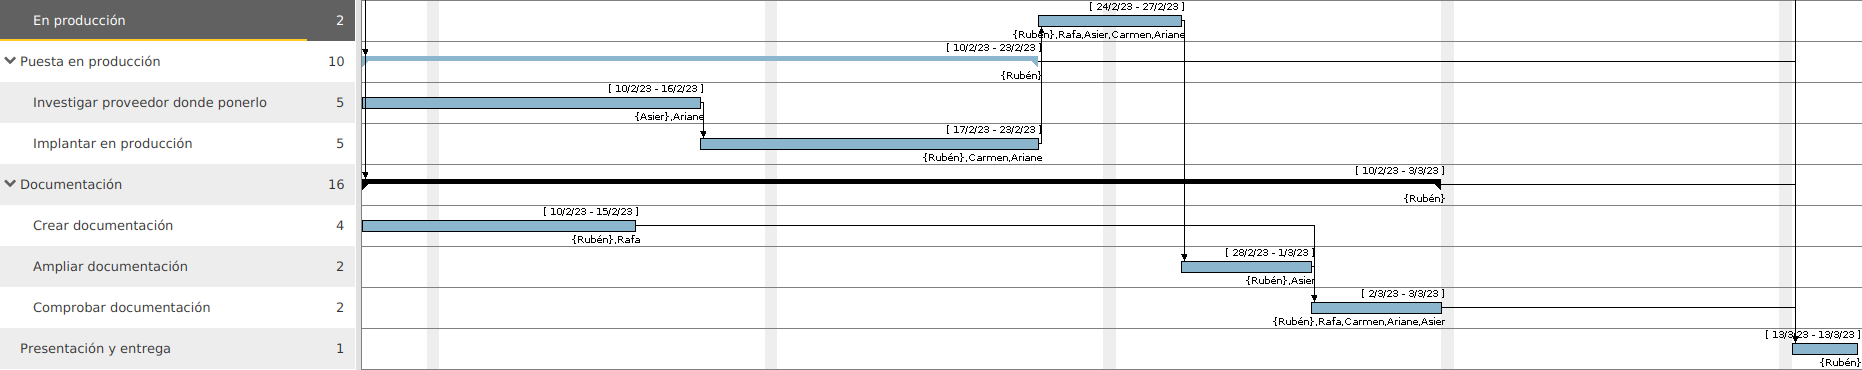
\includegraphics[frame,width=\linewidth]{img/gantt3.png}
\end{center}

Durante la investigación del proveedor, otra parte de los recursos comenzarán a hacer la documentación del proyecto realizado. Es importante dedicarle tiempo a la documentación ya que el cliente debe conocer lo realizado, las decisiones tomadas y el por qué de las mismas.

Se puede ver cómo tras la puesta en producción se van a utilizar 2 días para el “testo en producción”, y así confirmar que el proyecto funciona en producción como en el entorno de desarrollo.

Tras esto, se termina la documentación, añadiendo la parte de la puesta en producción y el equipo dedica un tiempo a comprobar que cumple con lo esperado.

Tal como se ha dicho previamente, desde la estimación de la última tarea a realizar hasta la presentación del proyecto se ha reservado una semana, para que en caso de que la estimación realizada no fuese muy precisa, contar con esos días de margen (junto con los otros días comentados anteriormente).


\chapter{Conclusiones}

La gestión de proyectos y la estimación de tiempos es una tarea compleja que requiere de experiencia para ser llevada a cabo de manera correcta. Es por eso que el usar aplicaciones que nos faciliten el trabajo debe ser obligatorio.

Por otro lado, aunque hoy en día se haga más uso de las metodologías ágiles a la hora de gestionar un proyecto, hemos comprobado que mediante el clásico diagrama de Gantt podemos realizar una primera estimación de tiempos que nos puede seguir siendo muy útil. Es por eso que es conveniente no olvidar este tipo de herramientas aunque usemos otras metodologías más modernas.

\end{document}
